\chapter{A Machine Learning Framework for Register Allocation}
\label{chap:ch5}

In this chapter, we will talk about MLRA - \textit{A Machine Leaning Framework for Register Allocation}. Its main objectives are the following: to perform semantically correct code generation,  to support multiple backend architectures, 
and to form proper communication between LLVM and ML model. 

The main focus of this work will be on the \textit{infrastructure development}. 

In section~\ref{sec:mlra:bg}, we will have an overview of Register Allocation and graph coloring problem. In section~\ref{sec:mlra:intro} and ~\ref{sec:mlra:pre_work}, we will talk about our proposal and the previous work respectively. In section~\ref{sec:mlra:components}, we discuss about different components of the framework like Capture Interference graph, ML model interface and Code generation. 



In Section~\ref{sec:mlra:arch}, we discuss about our Support for multiple architecture. 
In Section~\ref{sec:mlra:correct}, we present the correctness results.
In Section~\ref{sec:mlra:mlra_action}, we run the framework with an actual Model and report the (initial) results. 
In Section~\ref{sec:mlra:conclusion}, we will conclude this chapter also outlining the future work.



\section{Background}\label{sec:mlra:bg}
Register Allocation is an old and classic optimization problem. Many researchers provided many solutions for it, some exact solutions, but many heuristics as well. The success of a heuristic  depends upon the domain expertise of its developer. There is always a possibility that some important heuristics are missed, leading to sub-optimal performance.

The allocation should be done efficiently as the number of the registers is limited in number and may lead to poor performance if the registers are not assigned to a memory-bound variable properly. This leads to an increase in the use of the memory load and store operations. The memory operations are costlier than the register operations in case of performance. 

The popular register allocations are greedy, basic, fast, and pbqp register allocation. In this we are interested in the register allocation via Interference graph coloring. In the fig~\ref{fig:mlra-coloring}, there is a sample code for which we have the live interval interference chart. The Live interval are the scope of the variable when the variable was first defined and last used. Every variable has its own live interval and may interfere with other variable's live intervals. We can formulate this problem as the graph color program where the node is the variable or live interval and edges are the inference among the nodes. The Rule of Thumb, no two adjacent nodes be assigned the same color(register). The optimal graph coloring is a classic NP-Hard problem. 

\begin{figure}[t]
    \centering
    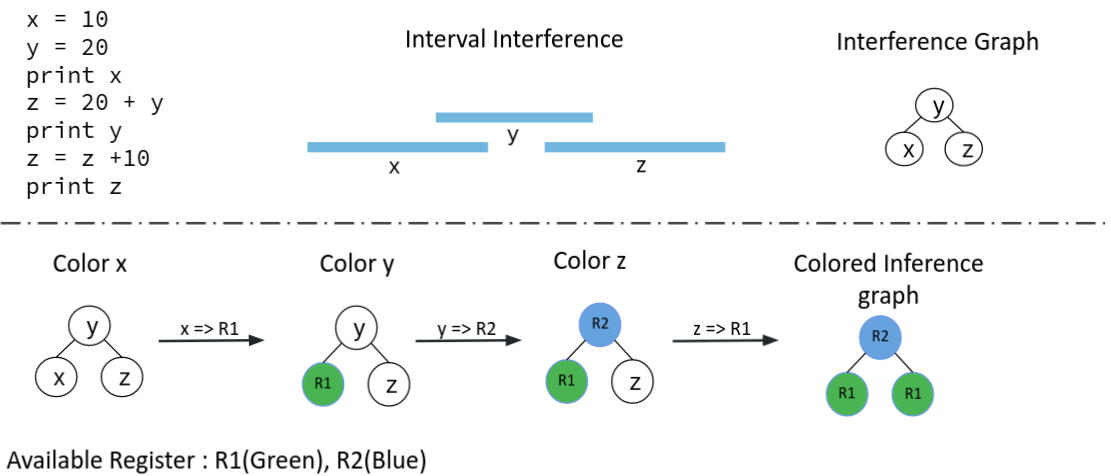
\includegraphics[scale=0.4]{figures/chapter-5/mlra_coloring.png}
    \caption{Register Allocation as Interference graph coloring}
     \label{fig:mlra-coloring}
\end{figure}
The LLVM has Greedy allocator  based on the graph coloring. There are four strategies used by this allocator respectively namely splitting, coalescing, eviction, and spilling (fig~\ref{fig:mlra-strat}). 

\paragraph{Splitting} - A selected node or live interval of the graph is divided into two sub-live intervals depending upon the point of splitting. The newly created live interval may or not form the edge between the existing nodes.

\paragraph{Coalescing} - In these two nodes which share the same variable value can be combined to form one node or single live interval. 

\paragraph{Eviction} - If some node of the graphs is already assigned a colored, but we wanted to uncolor the respective node. This process is known as eviction.

\paragraph{Spilling} - If the allocator ran out of register or heuristically suggests to assign the given variable to the memory. Memory load-store are costlier operations.

\begin{figure}[t]
    \centering
    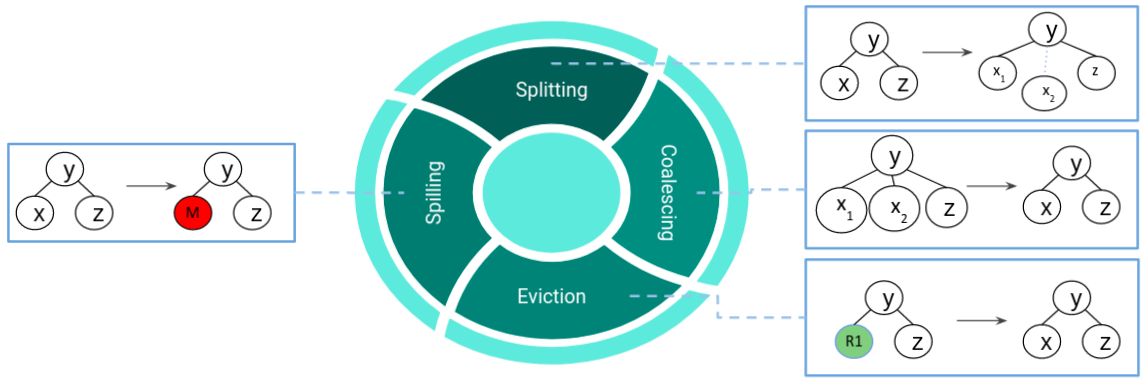
\includegraphics[scale=0.4]{figures/chapter-5/mlra_strategies.png}
    \caption{Register Allocation - Strategies}
     \label{fig:mlra-strat}
\end{figure}

The \textit{greedy allocator} uses all the four strategies in a heuristic manner and \textit{Basic allocator} uses splitting and spilling.

The current allocators are heuristically defined and provide sub-optimal solutions. Machine learning could help to improve the solutions.

\section{Introduction}\label{sec:mlra:intro}
We have developed a Machine learning framework for register allocation. It's main objectives are to perform semantically correct code generation, support multiple backend architecture and form proper communication between LLVM and ML model. The main focus of the work will be the infrastructure.

\section{Previous Work}\label{sec:mlra:pre_work}
\vk{More details before drawbacks}


In previous work by Das et al.~\cite{dlra:LLVMHPC_2020}, they tried to use the LSTM based deep learning model to predict the color (or register) for each node of the interference graph. The graphs with atmost 100 nodes are being supported by this work. \fixme{NOT CLEAR CLEANUP PLEASE}

There were several drawbacks to the above work. The solution was not integrated back to the LLVM pipeline. The proper modeling of the interference rule was not done. Because of this, the model could predict adjacent nodes to be assigned the same color, and this leads to incorrect register assignments. They have added a \textit{correction phase} to overcome this problem. Finally, the dataset used for the training was not realistic as it was sampled from random graphs using the graph based C library.

\begin{figure}[t]
    \centering
    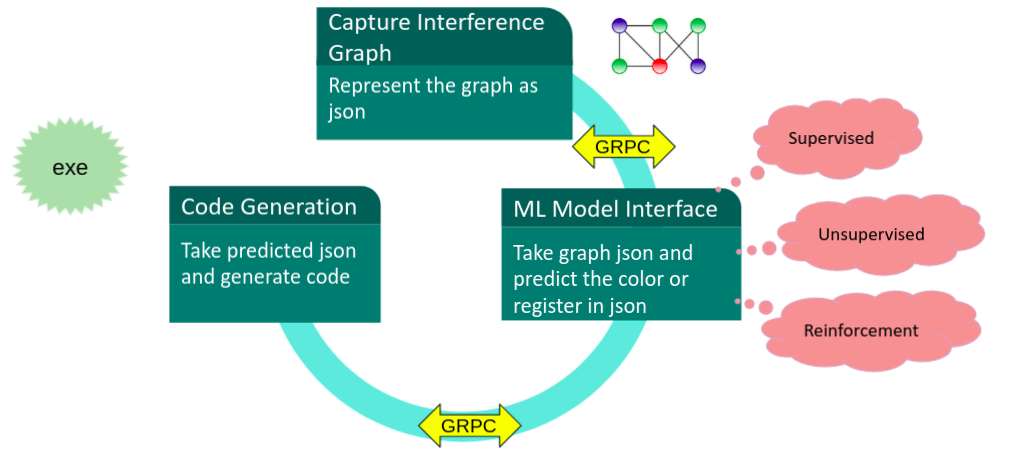
\includegraphics[scale=0.4]{figures/chapter-5/mlra_components.png}
    \caption{Components of correct ML based register allocation}
     \label{fig:mlra-components}
\end{figure}

\section{Framework Components}\label{sec:mlra:components}
The communication between the Capture interference graph, ML model, and code generation is done via gRPC~\cite{grpc}. The gRPC is a medium for cross-platform communication between C++ (LLVM) and Python (ML Model). See Fig.\ref{fig:mlra-components}
\subsection{Capture Interference Graph}
We have written a pass in LLVM which is responsible for capturing the interference graphs for the given input files. We annotate the graph with more information which would be later used by the other components. Fig.~\ref{fig:mlra-cig}.

The node comprises of node label, information regarding type of register physical or virtual, color and register Id if physical register, the class of the register, and embedding representation.

\begin{figure}[t]
    \centering
    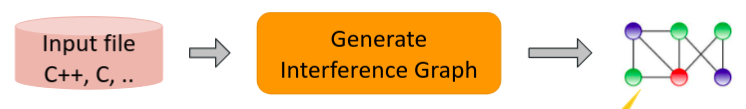
\includegraphics[scale=0.4]{figures/chapter-5/mlra_cig.png}
    \caption{Capture interference graphs}
     \label{fig:mlra-cig}
\end{figure}

The edge or interference that we are considering are between Virtual -- Physical registers and between Virtual -- Virtual registers. There are some physical register which are already in used and can’t be used to respect the interference rule, the edge is added. The Virtual -- Virtual is the trivial case.
\subsection{ML Model interface}
The Model interface could be any ML setting i.e. supervised, unsupervised, reinforcement and etc. The choice of the model depend upon the developer. The Model will be used in training as well as inference phase.

\subsubsection{Training}
From the previous Capture Interference graph component, we get the interference graphs and pass to the training paradigm. The interference graphs go to the model written in python where we request the LLVM to start the server through gRPC. After the server got started, the ML model runs and share its prediction with the CodeGen component through another gRPC call and receive some information as response. The response is used by model for it's proper execution. See Fig.~\ref{fig:mlra-training}.

\begin{figure}[t]
    \centering
    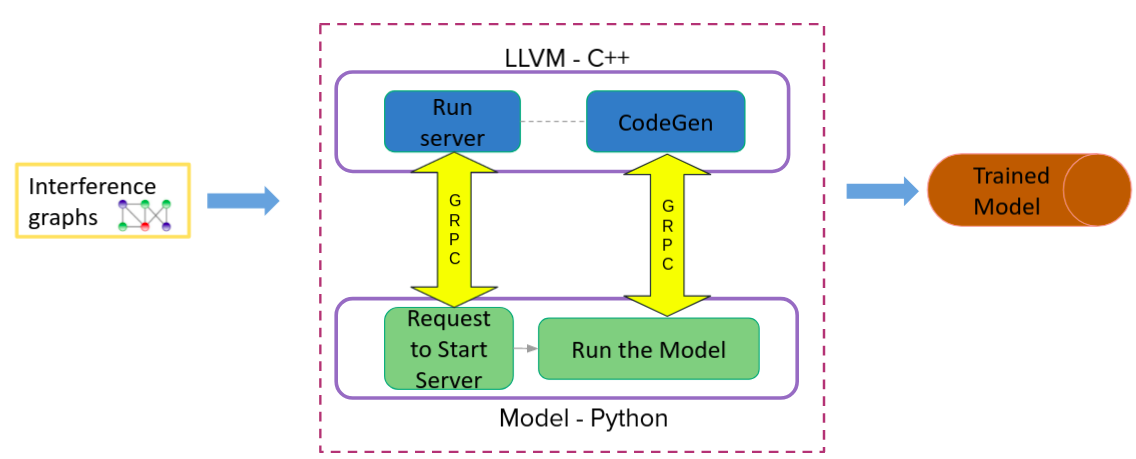
\includegraphics[scale=0.4]{figures/chapter-5/mlra_training.png}
    \caption{Train the model using gRPC}
     \label{fig:mlra-training}
\end{figure}

After all the interference graphs are visited, training is finished and the trained model used for the inference.
\subsection{Code generation or inference}
After the model is trained, we have added the integrated model with LLVM so that code generation could be done using the prediction suggested by the configured trained model.

While inference,the input file is given the LLVM and in the pipeline,  capture interference graph pass is invoke and the graph is then send to the Python through gRPC where it is feed to the trained model. The trained model send a color prediction json to the LLVM. In LLVM, the predicted colors/registers are mapped to the virtual registers and code is generated. See Fig.~\ref{fig:mlra-inference}.
\begin{figure}[t]
    \centering
    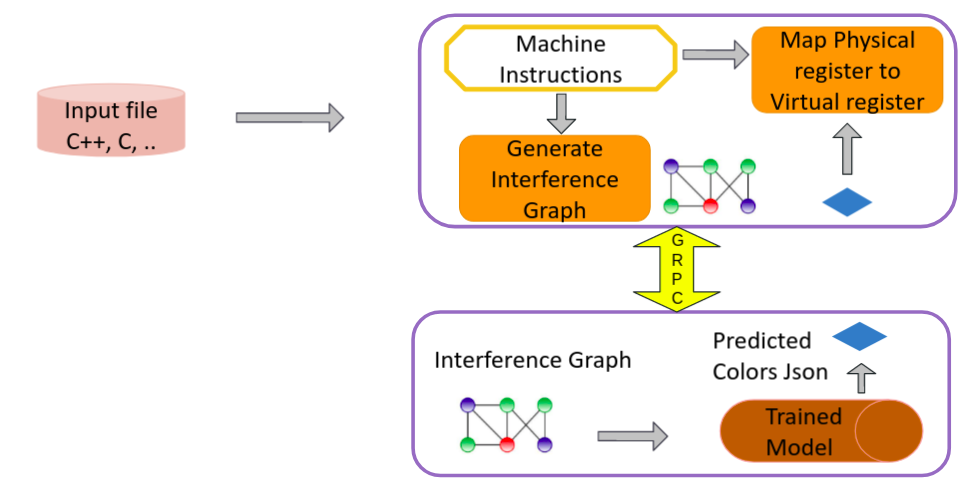
\includegraphics[scale=0.4]{figures/chapter-5/mlra_inference.png}
    \caption{Code generation using the trained model}
     \label{fig:mlra-inference}
\end{figure}

\section{Architecture}\label{sec:mlra:arch}
Different backends have their own instruction set and register set. In LLVM, this information is managed by TD files. TableGen takes the TD files and applies them to the backend so that this information is available at the code generation.

The TD files consist of information regarding different types of registers, classes information to which the register belongs, aliasing information, sub-registers details, and many more.
We have implemented a pass that captures information from the TD files and generates the configuration files which are used in different components. In the pass, we can configure the classes of the registers which we want to support, mapping between the color and the registers and overlapping information of the subregisters. 

These configuration files are used in the capture interference graph component to get the register id, color, register classes and other information. In the ML model inference, overlapping information, register color mapping configuration is used. Similarly in the code generation, color register mapping is used to get the color corresponding to the register.

\section{Correctness Results}\label{sec:mlra:correct}
To check the correctness of work framework, we have chosen GCC Torture benchmark. It is also part of llvm-testsuite. GCC Torture is a stress testing benchmark. For the experimentation, we have selected 1483 input files. We have selected two architectures X86 and AArch64 and successfully generated the code followed by successful execution.

For AArch64, we used QEMU\cite{qemu} to run the generated code on X86 machine. QEMU is a simulator or virtualization software that provide the libraries needed by assembly code of different architecture and executing on others. See the Tab.~\ref{tab:mlra:correction}.

% Please add the following required packages to your document preamble:



\begin{table}[h]
\begin{tabular}{llllll}
\hline
\textbf{Architecture} & \textbf{\begin{tabular}[c]{@{}l@{}}Program \\ files\end{tabular}} & \textbf{\begin{tabular}[c]{@{}l@{}}Base \\ compilable files\end{tabular}} & \textbf{\begin{tabular}[c]{@{}l@{}}Assembly\\ files generated\end{tabular}} & \textbf{\begin{tabular}[c]{@{}l@{}}Binary \\ files generated\end{tabular}} & \textbf{\begin{tabular}[c]{@{}l@{}}Successful \\ execution\end{tabular}} \\ \hline
\textbf{X86} & 1483 & 1483 & 1483 & 1483 & 1483 \\ \hline
\textbf{\begin{tabular}[c]{@{}l@{}}AArch64\\ (QEMU)\end{tabular}} & 1483 & 1479 & 1479 & 1479 & 1479 \\ \hline
\end{tabular}
\centering
\caption{Successful execution}
\label{tab:mlra:correction}
\end{table}

The errors undertaken will evaluating the framework are code generation error, linking error, runtime error, and semantic errors. A lot of iteration went into fixing these errors. We were able to achieve zero errors. See the Tab.~\ref{tab:mlra:error}.

\begin{table}[h]
\begin{tabular}{lllll}
\hline
\textbf{Architecture} & \textbf{\begin{tabular}[c]{@{}l@{}}Code \\ generation error\end{tabular}} & \textbf{Linking error} & \textbf{\begin{tabular}[c]{@{}l@{}}Runtime\\ error\end{tabular}} & \textbf{Semantic error} \\ \hline
\textbf{X86} & 0 & 0 & 0 & 0 \\ \hline
\textbf{AArch64} & 0 & 0 & 0 & 0 \\ \hline
\end{tabular}
\centering
\caption{Errors or Failures}
\label{tab:mlra:error}
\end{table}

\section{MLRA in Action}\label{sec:mlra:mlra_action}
Here we want to show how the framework can be used to register prediction using a naive reinforcement learning model on X86 architecture. We have taken 50K interference graphs from the SPEC 2017\cite{spec17-Bucek:2018:SCN:3185768.3185771} benchmarks. Embedding are generated using the IR2Vec on machine instructions representation(MIR). We are using reinforcement learning as the ML model interface and the objective of the model is to minimize the spill cost. The spill cost is the weight associated with each variable. Higher the value of spill cost more costly is load-store memory operations. See Fig.~\ref{fig:mlra-fw}

\begin{figure}[t]
    \centering
    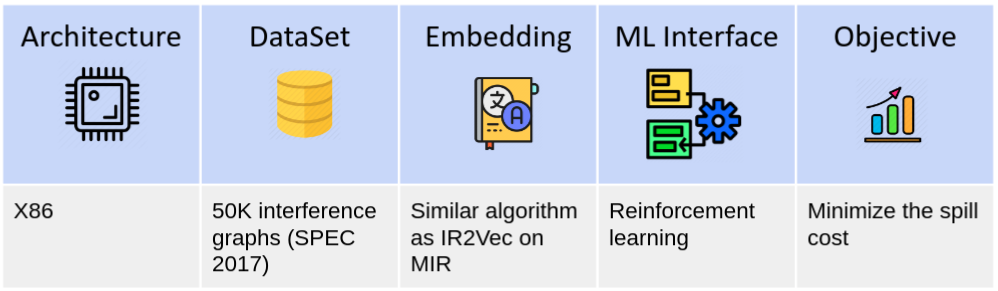
\includegraphics[scale=0.45]{figures/chapter-5/mlra_action.png}
    \caption{Framework configurations}
     \label{fig:mlra-fw}
\end{figure}

\subsection{Reinforcement Learning (RL) Model}
Reinforcement learning is the machine learning branch where datapoints do not have any label associated to them. During the training, a score is given to the model(agent) depending upon the intermediate and final action taken. The score is known as the reward which depend upon the action taken given an environment state. After applying action on the environment, its state or may not change. This change in the state would be good or bad. If the change is good, then a positive value is return as reward else negative value is returned as reward. The agent receive the reward from the environment and use this knowledge for future decision.

We have implemented a policy using the DQN algorithm in that the agent predicts which node should be assigned the register first.  While assigning the register, the policy is constraint by the interference rule. The objective of the model is to minimize the spillcost.

\subsection{Results}

Run the inference with trained model and showed our results on PolyBench and MiBench\cite{mibench}.
\subsubsection{PolyBench}
It is a Loop benchmark which have different computational intensive programs and a standard benchmark suites for polyhedral optimization. See the Fig.~\ref{fig:mlra-polybench} and Tab.~\ref{tab:mlra:polybench} for the performance comparison

\begin{figure}[h!]
    \centering
    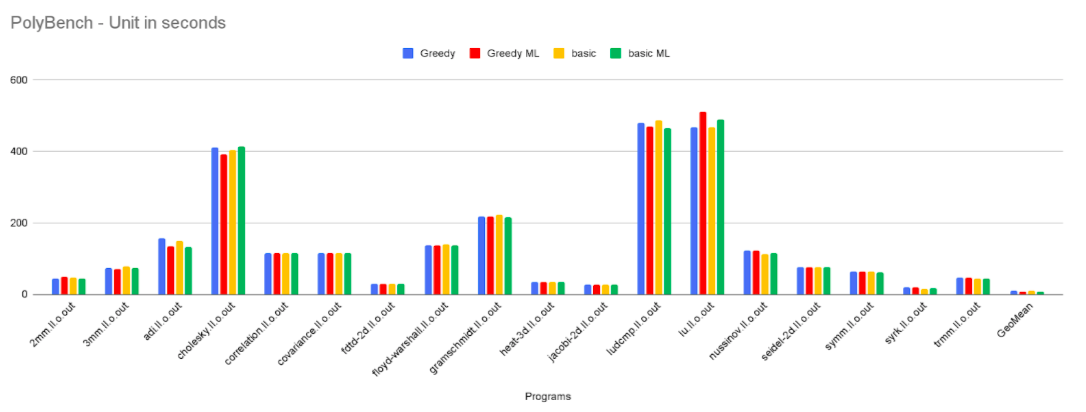
\includegraphics[scale=0.4]{figures/chapter-5/polybench.png}
    \caption{PolyBench - Runtime}
     \label{fig:mlra-polybench}
\end{figure}


\begin{table}[h!]
\begin{tabular}{|l|l|l|l|l|}
\hline
 & \textbf{Greedy} & \textbf{Greedy ML} & \textbf{Basic} & \textbf{Basic ML} \\ \hline
GeoMean & \multicolumn{1}{r|}{9.306} & \multicolumn{1}{r|}{9.050} & \multicolumn{1}{r|}{9.259} & \multicolumn{1}{r|}{8.891} \\ \hline
\end{tabular}
\centering
\caption{PolyBench - Runtime GeoMean}
\label{tab:mlra:polybench}
\end{table}

\subsubsection{MiBench}
This Benchmark is a micro-kernel benchmarks which are suitable for embedded devices.  See the Fig.~\ref{fig:mlra-mibench} and Tab.~\ref{tab:mlra:mibench} for the performance comparison

\begin{figure}[h!]
    \centering
    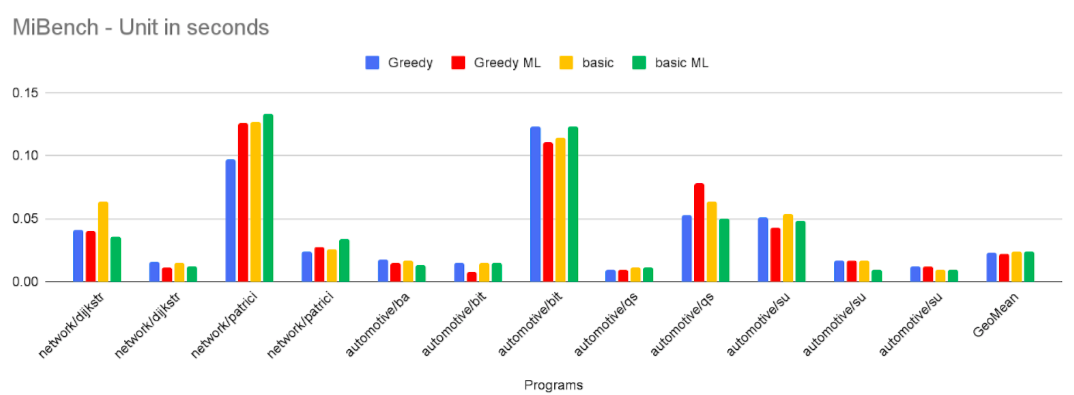
\includegraphics[scale=0.4]{figures/chapter-5/MiBench.png}
    \caption{Runtime - MiBench}
     \label{fig:mlra-mibench}
\end{figure}

\begin{table}[h!]
\begin{tabular}{|l|l|l|l|l|}
\hline
 & \textbf{Greedy} & \textbf{Greedy ML} & \textbf{Basic} & \textbf{Basic ML} \\ \hline
GeoMean & \multicolumn{1}{r|}{0.0227} & \multicolumn{1}{r|}{0.0220} & \multicolumn{1}{r|}{0.0242} & \multicolumn{1}{r|}{0.0237} \\ \hline
\end{tabular}
\centering
\caption{MiBench - Runtime GeoMean}
\label{tab:mlra:mibench}
\end{table}

\section{Conclusion}\label{sec:mlra:conclusion}
We have successfully developed a framework for register allocation which generates semantically correct code, which supports multiple architectures, and which can communicate between LLVM (in C++) and ML model (in Python).

This framework can also be used to support the ML based optimizations in LLVM for other optimization problems, in which such kind of information to-from is required.
